%! Licence = CC BY-NC-SA 4.0

%! Author = mariuszindel
%! Date = 30. Jan 2022
%! Project = Cheat-Sheet-Web-Engineering-3

\section{React}

\subsection{Einführung}
\begin{itemize}
    \item React ist eine Library, kein Framework
    \item Um User Interfaces zu bauen (,,The V in MV``)
\end{itemize}

\subsubsection{Prinzipien}
\underline{Komplexes Problem aufteilen} in einfache(re) \underline{Komponenten} für bessere \underline{Wiederverwendbarkeit} \underline{Erweiterbarkeit} \underline{Wartbarkeit} \underline{Testbarkeit}\\
\textbf{Aufgaben bei Entwicklung:} Beschreibung des UIs / Event-Handling / View Aktualisieren

\subsubsection{Komponente und Elemente}
Funktionen die ,,HTML`` zurückgeben (beliebige Komposition von React und DOM-Elementen)

\subsubsection{JavaScript XML}
\begin{minipage}{0.45\linewidth}
    React verwendet \highlite{cyan!50}{JSX} eine Erweiterung von \highlite{yellow!90}{JavaScript}. In \{\} stehen JavaScript-Expressions. Style-Attribute als Objekt angegeben!
\end{minipage}
\begin{minipage}{0.5\linewidth}
    \begin{center}
%    \vspace{-8pt}
        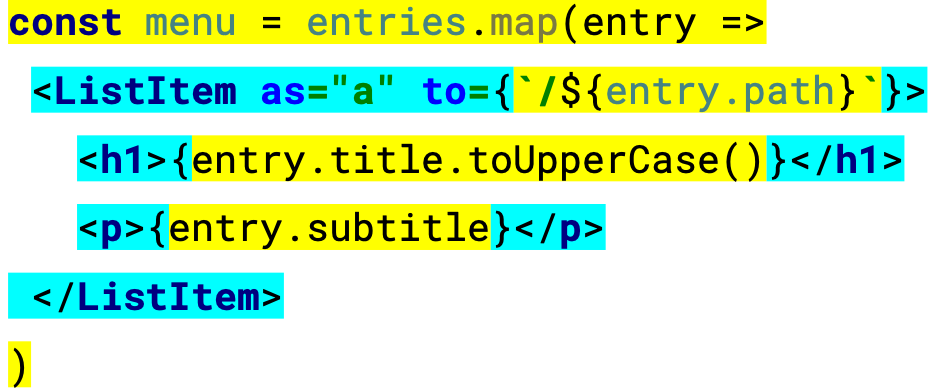
\includegraphics[width=1.14\linewidth]{./img/02-react/javascript_xml}
        \vspace{-8pt}
    \end{center}
\end{minipage}

\subsubsection{Props}
Komponenten erhalten alle Parameter/Properties als \textbf{props} Objekt.
\texttt{\tiny this.props} bei Klassen, bei Funktionen als Parameter. Immer \textbf{read-only}!

\subsubsection{Conditionals}
Was zu \underline{null}, \underline{true}, \underline{false} oder \underline{undefined} evaluiert wird nicht ausgegeben

\subsubsection{Desugaring (Entgiftung)}
JSX wird zu \textbf{React.createElement} vom Präprozessor gewandelt

\subsubsection{Rendering und Mounting}
Um Komponenten anzuzeigen $\rightarrow$ mounten

\begin{lstlisting}[style=JavaScript]
ReactDOM.render( <App/>,
    document.getElementById('root') )
\end{lstlisting}

\subsection{React State}
Veränderbarer Zustand von Komponenten. Ist immer privat. Ändert der State, wird auch die Komponente aktualisiert. Nur bei Klassen!
\begin{lstlisting}[style=JavaScript]
class Counter extends React.Component {
    state = { counter: 0 } }
\end{lstlisting}

\subsubsection{Event Handler}
\texttt{\tiny setState} nimmt Objekt und merged mit existierenden State. Nur angegebene Properties werden überschrieben! Können als Props an Komponenten weitergegeben werden.
\begin{lstlisting}[style=JavaScript]
increment = () => {
this.setState(state => ({counter: state.counter+1}))}
\end{lstlisting}

\subsubsection{Reconciliation (virtueller DOM)}
\begin{enumerate}
    \item Komponenten als virtueller DOM gerendert
    \item Wird state geändert, erstellt React virt. DOM
    \item Alter \& neuer DOM werden verglichen
    \item Geänderte DOM-Knoten im Browser erstellt
\end{enumerate}

\subsection{Formulare}
Event Handler (callback) bei den Inputs registrieren und Zustand ändern:
\begin{lstlisting}[style=JavaScript]
handleUsernameChange = (event) => {
  this.setState({username: event.target.value}) }
\end{lstlisting}
Verhindern, dass ganze Seite neu lädt
\begin{lstlisting}[style=JavaScript]
<form onSubmit={this.handleSubmit}> //(im HTML form)
handleSubmit = (event) => { event.preventDefault() }
\end{lstlisting}

\subsection{Komponenten Lifecycle}
Nur bei Komponenten als Klasse möglich!

\subsubsection{Mounting}
\textbf{1. constructor():} State initialisieren\\
\textbf{2. getDerivedStateFromProps():} Von state abhängige Props initialisieren.
\textbf{3. render()}\\
\textbf{4. componentDidMount():} DOM aufgebaut. Punkt um Async Daten zu laden. \texttt{\tiny setState} führt zu re-rendering.

\subsubsection{Updating}
\textbf{1. getDerivedStateFromProps():} Von state abhängige Props aktualisieren.
\textbf{2. shouldComponentUpdate():} render übersprungen bei false.
\textbf{3. render()}
\textbf{4. getSnapshotBeforeUpdate()}
\textbf{5. componentDidUpdate():} Analog zu DidMount, DOM ist aktualisiert.

\subsubsection{Unmounting}
\textbf{1. componentWillUnmount():} Aufräumen

\subsubsection{Error Handling}
\textbf{1. getDerivedStateFromError():} Error im state abbilden.
\textbf{2. componentDidCatch():} Logging, Verhindert porpagieren von Fehler.

\subsection{Container- \& Präsentations-Komponenten}
Trennung zwischen \underline{Container-} (render Methode) und \underline{Präsentations-} \underline{Komponenten} (nur Darstellung) [Wiederverwendung, Testing, Kopplung]

\subsection{React Router}
\begin{itemize}
    \item Zusätzliche Bibliothek (Komponentenbiblio)
    \item Komponenten anzeigen abhängig von URL
\end{itemize}

$\rightarrow$ Alle Routen müssen Teil des Routers sein.
\begin{lstlisting}
<Router>
\end{lstlisting}

$\rightarrow$ Component nur gerendert, wenn path matcht
\begin{lstlisting}
<Route exact path="/" component={Home} />
\end{lstlisting}

$\rightarrow$ App-interne Links verwenden \texttt{\tiny <Link>}
\begin{lstlisting}
<Link to="/">Home</Link>
\end{lstlisting}

$\rightarrow$ Wird ausgeführt, sobald gerendert
\begin{lstlisting}
<Redirect to="/somewhere/else">
\end{lstlisting}

\subsection{Hooks}
\textbf{Problem Lifecycle Methoden:} Code verteilt\\
\textbf{Problem Klassen-State:} State verteilt\\
\textbf{Fazit:} Ohne Klassen verständlicher. Mit Hooks Logik \& Zustand wiederverwenden

\subsubsection{State Hook}
\begin{lstlisting}
function Counter() {
    const [count, setCount] = useState(0); }
\end{lstlisting}
\textbf{Mehrere State-Variablen:} useState Aufrufe müssen immer in derselben Reihenfolge gemacht werden.

\subsubsection{Effect Hook}
\begin{lstlisting}
useEffect(() => { ... // Mount stuff
    return () => { ... // Unmount stuff
    } }, [] /* Dependencies ändern -> ausführen */);
\end{lstlisting}

\subsection{Typecheck}
\begin{itemize}
    \item Flow ergänzt JavaScript um Typ annotationen (können einfach ignoriert)
    \item TypeScript ist ein typisiertes Superset von JavaScript
\end{itemize}

\subsection{Redux}
Library für Statemanagement. State wird als Tree (immutable) von Objekten dargestellt. Veränderung am Tree führt durch den Reducer zu einem neuen Tree. State im \textbf{Store} verwaltet.

\subsubsection{Actions}
Benötigt um Stateänderungen zu machen. Wird an den Store \textbf{dispatched}. Action ist eine reine Beschreibung der Action.
\begin{lstlisting}
{type: 'TRANSFER', amount: 100 }
\end{lstlisting}

\subsubsection{Reducer (neuer State-Tree erstellen)}
Pure Funktionen, haben keine Seiteneffekte.
\begin{lstlisting}
function balance(state = 0, action) {
 switch (action.type) {
   case 'TRANSFER': return (state + action.amount);
   default: return state;  } }
\end{lstlisting}
\textbf{Reducer kombinieren:} Jeder Reducer erhält einen Teil des States, für den er zuständig ist. Resultat wird in neuem State-Objekt kombiniert.

\subsubsection{Store erstellen}
\begin{lstlisting}
const store = createStore(rootReducer);
\end{lstlisting}
Mit root-Reducer kann Store erstellt werden.

\subsection{Redux in React}
\texttt{\tiny mapStateToProps:} erhält State und kann daraus Props ableiten. Die Komponente bekommt auch die \textbf{dispatch Methode} des Stores als Prop. Komponenten werden durch \textbf{connect} mit Daten aus dem State-Tree versorgt. Store muss der Root-Komponente mitgegeben werden.

\subsubsection{Thunk Actions}
\textbf{thunkMiddleware:} Anstelle eines Objektes eine Funktion zu dispatchen (für asynchrone Actions). Store führt Thunk Action aus.

\subsubsection{Selectors}
Getter bei den Reducern, die einen Subtree des Stores zurückgeben. Wissen über den Aufbau des State-Trees bleibt bei den Reducern.
